
%% bare_conf.tex
%% V1.3
%% 2007/01/11
%% by Michael Shell
%% See:
%% http://www.michaelshell.org/
%% for current contact information.
%%
%% This is a skeleton file demonstrating the use of IEEEtran.cls
%% (requires IEEEtran.cls version 1.7 or later) with an IEEE conference paper.
%%
%% Support sites:
%% http://www.michaelshell.org/tex/ieeetran/
%% http://www.ctan.org/tex-archive/macros/latex/contrib/IEEEtran/
%% and
%% http://www.ieee.org/

%%*************************************************************************
%% Legal Notice:
%% This code is offered as-is without any warranty either expressed or
%% implied; without even the implied warranty of MERCHANTABILITY or
%% FITNESS FOR A PARTICULAR PURPOSE! 
%% User assumes all risk.
%% In no event shall IEEE or any contributor to this code be liable for
%% any damages or losses, including, but not limited to, incidental,
%% consequential, or any other damages, resulting from the use or misuse
%% of any information contained here.
%%
%% All comments are the opinions of their respective authors and are not
%% necessarily endorsed by the IEEE.
%%
%% This work is distributed under the LaTeX Project Public License (LPPL)
%% ( http://www.latex-project.org/ ) version 1.3, and may be freely used,
%% distributed and modified. A copy of the LPPL, version 1.3, is included
%% in the base LaTeX documentation of all distributions of LaTeX released
%% 2003/12/01 or later.
%% Retain all contribution notices and credits.
%% ** Modified files should be clearly indicated as such, including  **
%% ** renaming them and changing author support contact information. **
%%
%% File list of work: IEEEtran.cls, IEEEtran_HOWTO.pdf, bare_adv.tex,
%%                    bare_conf.tex, bare_jrnl.tex, bare_jrnl_compsoc.tex
%%*************************************************************************

% *** Authors should verify (and, if needed, correct) their LaTeX system  ***
% *** with the testflow diagnostic prior to trusting their LaTeX platform ***
% *** with production work. IEEE's font choices can trigger bugs that do  ***
% *** not appear when using other class files.                            ***
% The testflow support page is at:
% http://www.michaelshell.org/tex/testflow/



% Note that the a4paper option is mainly intended so that authors in
% countries using A4 can easily print to A4 and see how their papers will
% look in print - the typesetting of the document will not typically be
% affected with changes in paper size (but the bottom and side margins will).
% Use the testflow package mentioned above to verify correct handling of
% both paper sizes by the user's LaTeX system.
%
% Also note that the "draftcls" or "draftclsnofoot", not "draft", option
% should be used if it is desired that the figures are to be displayed in
% draft mode.
%
\documentclass[conference, letterpaper]{IEEEtran}
\usepackage{booktabs}
\usepackage{graphicx}
\usepackage[rflt]{floatflt}
\usepackage{frame, caption}
\usepackage{mathrsfs}
\usepackage{array}
\usepackage[cmex10]{amsmath}
\usepackage{color}
%
\usepackage{fancyhdr}
\usepackage[caption=false,font=footnotesize]{subfig}
\newcommand{\argmax}{\operatornamewithlimits{arg\,max}}

\hyphenation{op-tical net-works semi-conduc-tor}


\renewcommand{\thispagestyle}[2]{} 


\fancypagestyle{plain}{
        \fancyhead{}
        \fancyhead[C]{first page center header}
        \fancyfoot{}
        \fancyfoot[C]{first page center footer}
}
\pagestyle{fancy}


\headheight 20pt
\footskip 20pt

\rhead{}

%Enter the first page number of your paper below
\setcounter{page}{1}

%Header
\fancyhead[R]{\textit{Intelligent Systems Conference 2018 \\ 6-7 September 2018 $|$ London, UK}}
\renewcommand{\headrulewidth}{0pt}

%Footer
\fancyfoot[C]{IEEE}
\renewcommand{\footrulewidth}{0.5pt}
\fancyfoot[R]{\thepage \  $|$ P a g e }


\begin{document}

%
% paper title
% can use linebreaks \\ within to get better formatting as desired
\title{I've got the power's value! A computational model to evaluate the interlocutor's behaviors in collaborative negotiation}


% author names and affiliations
% use a multiple column layout for up to three different
% affiliations
\author{\IEEEauthorblockN{Michael Shell}
\IEEEauthorblockA{School of Electrical and\\Computer Engineering\\
Georgia Institute of Technology\\
Atlanta, Georgia 30332--0250\\
Email: http://www.michaelshell.org/contact.html}
\and
\IEEEauthorblockN{Homer Simpson}
\IEEEauthorblockA{Twentieth Century Fox\\
Springfield, USA\\
Email: homer@thesimpsons.com}
\and
\IEEEauthorblockN{James Kirk\\ and Montgomery Scott}
\IEEEauthorblockA{Starfleet Academy\\
San Francisco, California 96678-2391\\
Telephone: (800) 555--1212\\
Fax: (888) 555--1212}}

% conference papers do not typically use \thanks and this command
% is locked out in conference mode. If really needed, such as for
% the acknowledgment of grants, issue a \IEEEoverridecommandlockouts
% after \documentclass

% for over three affiliations, or if they all won't fit within the width
% of the page, use this alternative format:
% 
%\author{\IEEEauthorblockN{Michael Shell\IEEEauthorrefmark{1},
%Homer Simpson\IEEEauthorrefmark{2},
%James Kirk\IEEEauthorrefmark{3}, 
%Montgomery Scott\IEEEauthorrefmark{3} and
%Eldon Tyrell\IEEEauthorrefmark{4}}
%\IEEEauthorblockA{\IEEEauthorrefmark{1}School of Electrical and Computer Engineering\\
%Georgia Institute of Technology,
%Atlanta, Georgia 30332--0250\\ Email: see http://www.michaelshell.org/contact.html}
%\IEEEauthorblockA{\IEEEauthorrefmark{2}Twentieth Century Fox, Springfield, USA\\
%Email: homer@thesimpsons.com}
%\IEEEauthorblockA{\IEEEauthorrefmark{3}Starfleet Academy, San Francisco, California 96678-2391\\
%Telephone: (800) 555--1212, Fax: (888) 555--1212}
%\IEEEauthorblockA{\IEEEauthorrefmark{4}Tyrell Inc., 123 Replicant Street, Los Angeles, California 90210--4321}}




% use for special paper notices
%\IEEEspecialpapernotice{(Invited Paper)}




% make the title area
\maketitle


\begin{abstract}
%\boldmath
Interpersonal dominance relation has a major effect on the outcome of a negotiation. It has been shown that when participants adopt complementary dominance behaviors (one being dominant and the other being submissive), they reach mutually beneficial outcomes and this increases their reciprocal likings. In this paper, we investigate about the simulation of this interpersonal relationship in the context of collaborative negotiation between artificial agents.

Our simulation is based on a previously published model. We present a Theory of Mind model that allows an agent to evaluate its interlocutor's level of dominance. The agent establishes the relation of dominance by adapting its behavior of power to complement the power of its interlocutor. We show on agent-agent simulation that the system correctly predicts the interlocutor's power. 
\end{abstract}
% IEEEtran.cls defaults to using nonbold math in the Abstract.
% This preserves the distinction between vectors and scalars. However,
% if the conference you are submitting to favors bold math in the abstract,
% then you can use LaTeX's standard command \boldmath at the very start
% of the abstract to achieve this. Many IEEE journals/conferences frown on
% math in the abstract anyway.

% no keywords


\begin{IEEEkeywords}
	
	Human agent interaction ; Collaborative negotiation; Interpersonal relation of power;Reasoning about other; Theory of mind
\end{IEEEkeywords}


% For peer review papers, you can put extra information on the cover
% page as needed:
% \ifCLASSOPTIONpeerreview
% \begin{center} \bfseries EDICS Category: 3-BBND \end{center}
% \fi
%
% For peerreview papers, this IEEEtran command inserts a page break and
% creates the second title. It will be ignored for other modes.
\IEEEpeerreviewmaketitle

\section{Introduction}
Negotiation is a common task in daily life. People negotiate not only in professional situations (\emph{e.g.} for a salary increase or a promotion) but also in more simple situations such as choosing the movie to watch or the holiday destination. In the last decade, a variety of conversational agents have been created to negotiate with people [refs]. Theses agents are designed with a growing number of decisional abilities, including multi-party and multi-issues negotiation capabilities.

However, negotiation is a multifaceted process which also involves social interaction and affects as well as personal preferences and opinions  \cite{bro2010affective}. Several research considered the role social behavior in the negotiation process. For instance, [ref-marsella] studied the impact of emotion on the outcome of the negotiation. [ref-elisabetta] studied how the expression of social attitudes at the non-verbal level changes the perception of the negotiation.

One key element in the social aspect of negotiation is the interpersonal relation between the participants. Indeed, researches in social psychology demonstrated that the relation of dominance affects the way the negotiation process is perceived \cite{van2006power}. Negotiating parties often differ in terms of dominance and this difference exerts an important influence on the behavior of participants. Negotiators build different negotiation strategies depending on their relative dominance. This directly influences the outcomes of the negotiation. More precisely, Tidens \cite{tiedens2003power} showed that dominance complementarity (\emph{i.e.} one negotiator exhibits dominant behaviors while the other one responds with submissive ones) leads the negotiators to reach mutually beneficial outcomes and increases their reciprocal likings. \cite{wiltermuth2015benefits,tiedens2003power}.

For this reason, it is important to develop negotiator agents that can adapt their social behavior to the dominance of their interlocutor. Our work aims at developing such a system that is capable of evaluating and adapting to this degree of dominance.

We focus on a specific kind of interaction called \emph{collaborative negotiation}. Unlike adversarial negotiation, collaborative negotiation assumes that each participant is driven by the goal of finding a trade-off that best satisfies the interests of all the participants as a group, instead of one that maximizes his own interest\cite{sidnerartificial,chu1995response}. In order to develop our adaptative negotiator agent, we first designed a model of collaborative negotiation that allows an agent to express its social dominance through negotiation strategies \cite{ouali2017computational}. We showed that human observers correctly perceive the dominance expressed by the agent. The next steps are to evaluate the level of dominance of the interlocutor and to adapt the agent's level of dominance. In this paper, we present a theory of mind approach to evaluate the level of dominance of the interlocutor (step 2 on Figure~\ref{fig:schema-general}).

%	
%	
%	 that allows the agent to establish a complementary relation of dominance with the user. Thus, the agent adapts its behaviors to complement the behaviors of the user. 
%	
%	To construct a complementary relation of dominance, the agent has to predict the user's behaviors of power in order to adapt a complementary strategy. 
%	%il manque qlq chose
%	In a previous work \cite{ouali2017computationall}, we designed a negotiation agent capable of expressing negotiation's strategies that reflect his level of power. We propose to extend this model, with theory of mind abilities based on simulation, that allow the agent to simulate the decisional model of tis partner and predict his level of dominance.
%	
%	Since the implemented behaviors of power reflect human behaviors, we assume that the user uses the same decision model to negotiate. Therefore, the agent will define beliefs about the user's reasoning model based on the utterances expressed. 
%	
%	
%	In this paper specifically, we present our model of theory of mind that constructs a mental model of the user and processes the value of power he exhibits in the negotiation. 
%	
The paper is organized as follows. Section II gives an overview of previous automated negotiation agents with theory of mind and other related work on social behavior recognition. In section III, we briefly present our model of dialogue for collaborative negotiation. We show that extendeding this model with a theory of mind raises computational issues. We propose a new model to evaluate the dominance of the interlocutor. This model is based on reasoning with uncertainty. Section IV presents an evaluation of this new model in the context of agent-agent negotiation. We show that the system correctly predicts the interlocutor's power in spite of the restrictions on the model. In section V, we discuss the future use of this new model for building an adaptative negotiator agent.


\section{Related works}

In social interactions and negotiation in particular, reasoning about the beliefs, goals, and intentions of others is crucial. People use this so-called theory of mind \cite{premack1978does} or mentalizing to understand why others behave the way they do, as well as to predict the future behavior of others. Therefore, various negotiation models use theory of mind approaches to create  more realistic models of negotiation. 

For instance, Pynadath \textit{et al}\cite{pynadath2013you} showed the advantages of theory of mind on negotiation even with an overly simplified model. They observed significant similarities between	the partner behaviors and the agent's idealized expectations. Moreover, deviations in expectations about the other did not affect the agent performances and played in some cases in the advantage of the agent.

De Weerd \textit{et al} \cite{de2013higher} also investigated the use of high-order theory of mind in mixed-motive situations where cooperative and competitive behaviors play an important role. They found that the use of first-order and second-order theory of mind allow agents to balance competitive and cooperative	aspects of the game. This prevents agents from breaking down compared to  agents without theory of mind.


Both approaches only focus on rational behaviors and exclude social aspects. However, the impact of social behaviors has been extensively debated in social psychology. Among such works, various researches have been investigating emotion recognition in negotiation; the effects of one individual's	emotions on the other's social decisions and behavior during the negotiation. Moreover, they investigate how theses resource of information are integrated.
For example, Elfenbein\textit{ et al} \cite{elfenbein2007reading} proved that  emotion recognition accuracy is positively correlated to  better performances in negotiation

In the same vein, several researches suggested that anger expression has effects on the negotiation \cite{sinaceur2006get,van2010interpersonal,ferguson2004social}. For example, VanKleef \cite{van2004interpersonal} demonstrated that negotiators monitor their opponent's emotions and use them to estimate the opponent's limits, and modify their demands according to the presumed location of those limits. As a result, negotiators concede more to an angry opponent than to a happy one. 


For theses reasons, reasoning about the social behaviors is important for the percpective of constructing negotiators agents. \cite{alfonso2015emotional} proposed a model that can observe and predict other's agents emotional behaviors. The three step method proposes to revise the agent's  beliefs by integrating a Bayesian model which infers probabilities about the emotional behaviors of other's agents and compute probabilistic prediction about their appraisals.

Marcella \textit{et al} \cite{klatt2011negotiations} proposed a model of negotiation in the context of aid prevention. The model tries to combine handling of emotions with general structures of negotiations. 

In the context our work, we focus on the impact of dominance in the negotiation. Dominance as an interpersonal relation is defined by burgoon \cite{burgoon1998nature} as expressive, relationally based communicative acts by which power is exerted and influence achieved. Furthermore, it is a dyadic variable in which control attempts by one individual are accepted by the
interactional partner \cite{dunbar2005perceptions}. For this reason, we focus on dominance complementarity between a negotiator agent and a human user in the context of collaborative negotiation. 

Dominance complementarity is characterized by one person in a dyadic interaction behaving dominantly and his counterpart behaving submissively \cite{tiedens2003power} and those behaviors have been investigated in the context of negotiation. \cite{tiedens2003power} showed that when complementarity occurs in an interaction, people feel more comfortable and helps to create interpersonal liking relation.
Moreover, \cite{wiltermuth2015benefits} showed that dominance complementarity can positively improve coordination and by consequences improve objective benefits.

Our goal is to create a model of negotiation in which the agent adapts its negotiation strategies to the relation of dominance established with the user. Therefore, the agent has to reason about user's behaviors of \emph{power} to understand the level of dominance or submissiveness expressed. The agent then adopt a complementary strategy in order to complement the user behaviors and establish the relation of dominance.

We present in this paper a model of theory of mind that builds beliefs about the user behaviors of power in order to predict his behavior of dominance. We propose to use our model of negotiation based on power in order to reason about the user behaviors. 


\section{Model of collaborative negotiation}

Our simulation of interpersonal relation of dominance is based on a previously proposed model of collaborative negotiation \cite{x}. In this model, the artificial agent selects an utterance based on the previously exchanged information and on its personal level of social power, represented as a variable in [0,1]. We showed that the dialogues produced by this model allow human users to correctly perceive the different dimensions of social power expressed by the agent.

Our goal is to use this dialogue model to simulate the interlocutor's behavior. From a given utterance produced by the interlocutor, the agent will try to evaluate the level of power by comparing this utterance with the possible outcomes of the dialogue model.

It is not necessary to have a complete knowledge of this dialogue model to understand the simulation presented here. However, some elements are required to explain our approach. This section briefly presents the main principles of the collaborative negotiation dialogue model.

\subsection{Dialogue model}

%	We defined a dialogue system of collaborative negotiation which enable  a conversational agent to create and adapt its negotiation strategy to the power it intends to express. 
The goal of a negotiation is to choose an option in a set of possible values $\mathcal{O}$. Each option $o\in\mathcal{O}$ is defined as a set of values $\{v_1, ..., v_n\}$ associated to criteria $\{C_1, ..., C_n\}$ that reflect the options characteristics.  For instance, in a negotiation about restaurants, the criteria might be the type of cuisine and the price, we could have the option: $(French,expensive)$.

The agent is provided with a set of partial or total ordered preferences $\prec_i$ defined for each criterion $C_i$. For example, the agent prefers Chinese food to Turkish one. Using theses preferences, it can compute a score of satisfaction $sat(v)$ for each value of each criterion. The satisfaction of a value $v \in C_i$ is computed as the number of values that the agent prefers less in the preferences order $\prec_i$.
%, then, the score is normalized in $[0, 1]$: 

%	\begin{equation}
%	sat(v, \prec_i) =	1 - \left( \frac{|\{v' : v' \neq v \  \wedge \ (v \prec_i v')\}| }{( |C_i| - 1 )}\right)
%	\end{equation}
%	
The notion of satisfaction represents the score of liking for the value. The closer the satisfaction of a value $v$ gets to 1, the more the agent likes $v$.

\par For example, let us consider a domain $D =\{A, B, C, D\}$ with the set of preferences $\{A \prec B, C \prec D , B \prec D \}$. The values of satisfiability are depicted in the table \ref{tab:sat}.
\begin{table}
	\centering
	\begin{tabular}{ |c|c|c|c|c| }
		\hline				
		value & A & B & C & D \\
		\hline
		
		\hline
		sat(value) & 0.3 & 0.6 & 0.6 & 1 \\
		\hline
		
	\end{tabular}
	\caption{Value of satisfiability for the model $D$.}
	\label{tab:sat}
\end{table}

\par
In our model, agents communicate using 5 utterances types: \emph{AskPreference} and \emph{StatePreference} to exchange information about the preferences; \emph{Propose}, \emph{Accept} and \emph{Reject} to make negotiation moves. The selection of these utterance types and the values is based on the decision model related to power presented hereafter.

\subsection{Decision based on power}

The decisional process is built to take into account the power of the agent, its preferences and the context of the negotiation. Therefore, the agent is initiated with a value of power $pow \in [0,1]$. 

The selection of the utterance relies on three elements.

\subsubsection{Lead of the dialogue}
\cite{magee2007power,de2004influence} showed that the participant with higher power tends to lead the dialogue and to focuses on the negotiation convergence. In our model, this means that agents with high values of power ($pow>0.5$) will selected negotiation moves preferably. On the contrary, submissive negotiators focus on having accurate knowledge about the other to take the fairest decision. In our model, agents with low power will select StatePreference and AskPreference utterances more often.

\subsubsection{Satisfiability: StatePreferences}
\label{sec:sat}
When using a \emph{StatePreference(v)} utterance, the agent expresses its liking for a value. As showed by \cite{de1995impact}, high-power negotiators are more demanding than low-power ones. For this reason, in our model, the set of values that the agent likes, named $S$, depends on the level of power $pow$. It is computed as follows:
\begin{equation}
\forall v,\hspace{2mm} v\in S\hspace{2mm}\mathrm{iff}\hspace{2mm}sat(v) \geq pow
\end{equation}

For example, if we consider the preference set given on table~\ref{tab:sat} and the power $pow=0.6$, we can compute the set of satisfiable values $S = \{B, C, D\}$. This set $S$ is used directly to compute the values of \emph{StatePreference} utterances.	

\subsubsection{Acceptability: negotiation moves}
During the negotiation, the agent makes decisions about the proposals it receives. It might express an \emph{Accept} or \emph{Reject}. However, when the negotiation is not converging, the agent has to make concessions which means that the agent has to lower his level of demand.

\begin{floatingfigure}[r]{1.5in}
	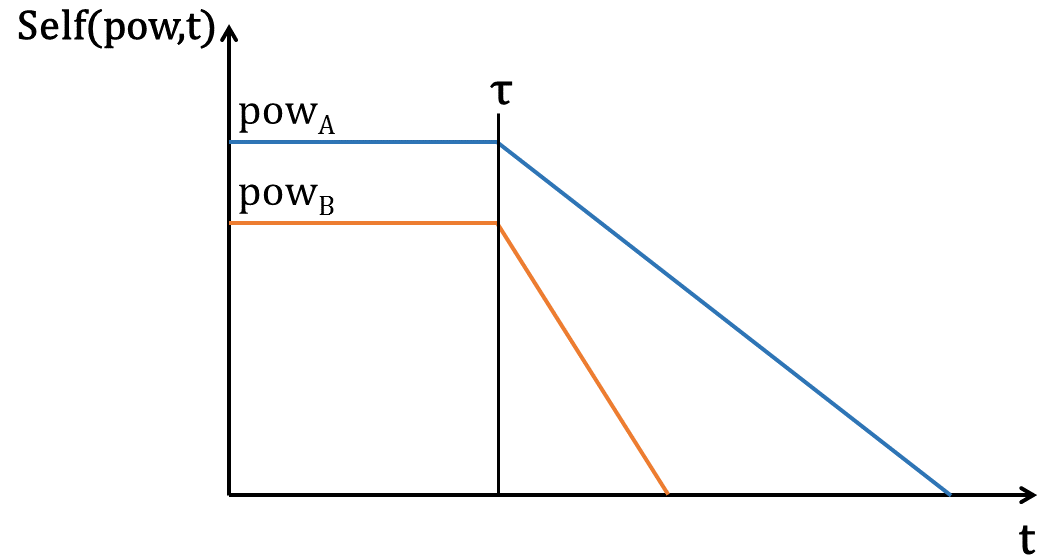
\includegraphics[width=1.5in]{figs/sv3.png}
	\caption{\label{fig:conc}Concession curve}
\end{floatingfigure} 

We compute the notion of concession with $self(t)$, which is a time varying value of $pow$ that decreases over time $t$. In the beginning, $self(0) = pow$, when the negotiation evolves without converging self decreases $self(t) < pow$ as presented in the figure \ref{fig:conc}.

Thus, a proposal with a value $v \in C_i$ is \emph{acceptable} ($v \in Ac$) is computed with a boolean function:
\begin{equation}
acc(pow, v) = sat(v, \prec_i) \geq self(t)
\end{equation}	
and we note $Ac$ the set of acceptable values.

%When negotiation progress in time without converging to a trade-off,
As the negotiation evolves, the agent might accept proposals which are not satisfiable, as a consequence of making concessions. We note $M$ the set of not-satisfiable values that can be accepted in the current dialogue move.

$\{v \in M / v \in Ac, v \notin S\}$.

%	Therefore, in order to accept \emph{Accept} or propose \emph{Propose} a value $v$, this value has to be acceptable $v \in Acc$. In the contrary, a value $v$ can be rejected (\emph{Reject}) if $v \not \in Acc$ and by consequences $v\not \in S$
%	



XXX

Table~\ref{tab:utt} presents the applicability condition for each utterance.

\begin{table}
	\centering
	\begin{tabular}  {|l|l|}
		\hline
		Utterance & Applicability condition \\
		\hline
		StatePreference(v) & $sat(v, \prec_i) \geq pow$ \\
		\hline 
		Propose(v) & $acc(pow, v) = true$ \\
		\hline
		Accept(v)  & $acc(pow, v) = true$ \\
		\hline
		Reject(v) & $acc(pow, v) = false$ \\
		\hline
	\end{tabular}
	\caption{Value of satisfiability for the model $D$.}
	\label{tab:utt}
\end{table}

\subsection{Beliefs about other}

In order to build a complementary relation of dominance with the user, the agent has to construct beliefs about the behaviors of power expressed by the user and adapt to complement his behavior as presented in figure \ref{fig:model}.

\begin{figure*}
	\fbox{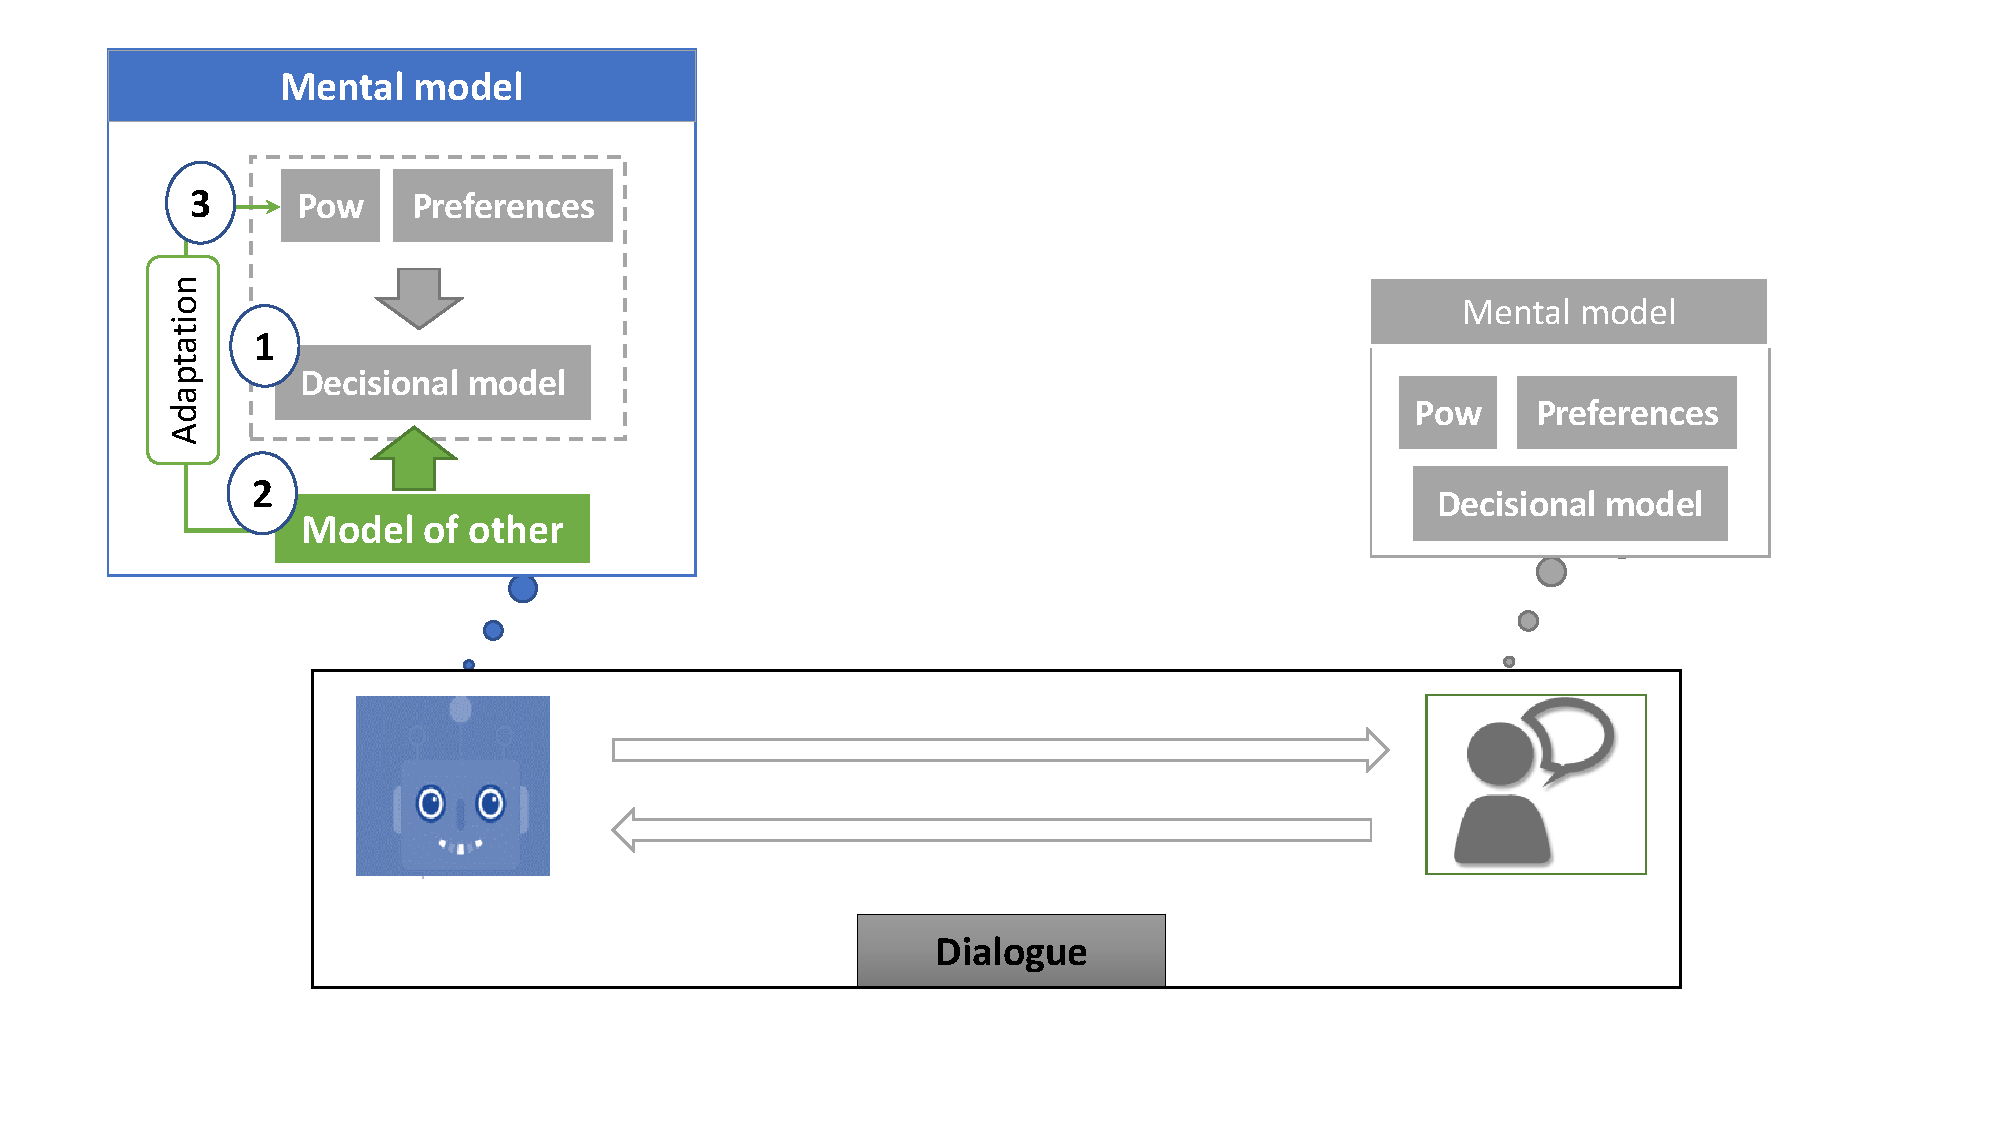
\includegraphics[width=\linewidth, height= 0.4\textheight]{figs/model_tom.pdf}}
	\caption{Model of collaborative negotiation with a model of other} 
	\label{fig:model}
\end{figure*} 

We make the assumption that our model of dialogue effectively presents the process of utterance's selection using power. 

Based on this assumption, we propose to enable the agent with a model of theory of mind based on simulation \cite{bibid}. The agent uses its model of decision in order to guess the behavior of the user from its enunciated utterance.   

The agent needs to infer hypotheses about the user's mental state (\emph{i.e} Pow, Preferences) in order to reason about his behaviors. With knowledge gathered during the negotiation, the agent will remove inconsistent hypotheses.

First, we define hypotheses about the possible values of $pow$ that the agents aims to predict. Let $H_{pow} = \{0.1, 0.2, \ldots, 0.9\}$ be the hypotheses on $pow$.

Second, for each fixed hypothesis $ h_i \in H_{pow}$, we define hypotheses on the different set of preferences  noted $M_H $. Thus, for each criterion $C_i$ of the a topic , we compute all the possible combination of preference's relations. When relations of preferences are total ordered, the total number of preference's relations is in the order of $|H{C_i}| = |C_i|!$. In the case of partial ordered relations of preferences, the total number of possible relations is  $ |H{C_i}| = (|C_i| + 1)!$. Hence, for a topic of negotiation with $n$ criteria, the number of possible set of preferences is 
$$ |M_H| = \prod_{i=1}^n (|H{C_i}|)$$ 

For each hypothesis $ h_i \in H_{pow}$, we associate the set of possible preferences $M_H(h_i)$ identical for all the hypotheses in the beginning. After each user's turn, the agent updates its hypotheses and remove the ones that did not produced the same utterance than enunciated by the user. The value of power selected is computed as follow:

\begin{equation}
pow_{Other} = \operatorname*{arg\,max}_{h_i \in H_{pow}} (M_H(h_i))
\end{equation} 

This solution presents a computational limitation concerning the number of hypotheses formulated to generate the preferences. As presented, the size of hypotheses $M_H$ is considerable which can slow down the dialogue generation. However, we don't aim to know the "correct" preferences of the user but only the expressed power $pow$. 

To deal with this limitation, we propose to infer hypotheses with partial knowledge about preferences. We only need to represent information about the user's preferences to be able reproduce its decisional model. 



\subsection{Partial model of preferences}

The model of preferences is used to compute the satisfiability of values (see section \ref{sec:sat}). Knowing the set of satisfiable values is crucial for the decisional process. Therefore, instead of computing hypotheses on the set of preferences, we propose to compute hypotheses about $S$, the set of satisfiable values for a giving value of power $pow$.  

\par In order to generate theses hypotheses for any criterion, we make the strong assumption that preferences are \emph{total ordered.} In this case, all the values are comparable and could be ranked by order of preferences. Knowing the rank of preferences allows the agent to compute in advance the possible values of satisfiability.

For example, the criterion $D$, of the size  $|D| = 4$ with total ordered preferences, get the values of satisfiability as presented in table \ref{tab:poss}.
\begin{table}[h]
	\centering
	\begin{tabular}{ |c|c|c|c|c| }
		\hline				
		rank(value) & 1 & 2 & 3 & 4 \\
		\hline
		Nb predecessors & 3 & 2 & 1& 0 \\
		\hline
		Sat(value) & 0 & 0.33 & 0.66 &1 \\
		\hline
		
	\end{tabular}
	\caption{Values of satisfiability for the criterion $D$.}
	\label{tab:poss}
\end{table}

Based on the values of satisfiability, and given a fixed value of $h_i \in H_{pow}$, we can compute the size of $S$ in order to generate hypotheses on the different combination of satisfiable values  noted $M_h(h_i)$. For example, considering a value of $pow =0.6$, and the same criterion $D$, the number of satisfiable values $|S| = 2$. Therefore, $M_h(pow) = \{(A,B), (A,C), (A,D), (B,C), (B,D), (C,D)\}$. This process is generalized to all the hypotheses of $H_{pow}$. An example is presented in the table \ref{tab:sat}




\begin{table}[h]
	\centering
	\begin{tabular}{ |c|c|c| }
		\hline
		& \multicolumn{2}{c|}{Hypotheses}  \\
		\hline
		Hypothesis & pow & $M_h(pow)$ \\
		\hline
		H1&0.3&$\{ (A,B,C) , (A,B,D), (A,C,D), (B,C,D) \}$ \\
		\hline
		H2&0.4&$\{ (A,B), (A,C), (A,D), (B,C), (B,D), (C,D) \}$ \\
		\hline
		H3&0.5&$\{ (A,B), (A,C), (A,D), (B,C), (B,D), (C,D) \}$\\
		\hline
		H4&0.6&$\{ (A,B), (A,C), (A,D), (B,C), (B,D), (C,D) \}$ \\
		\hline
		H5&0.7&$\{ (A), (B), (C), (D) \}$\\
		\hline
		H6&0.8&$\{ (A), (B), (C), (D) \}$ \\
		\hline
		H7&0.9&$\{ (A), (B), (C), (D) \}$ \\
		\hline
	\end{tabular}
	\caption{Hypotheses on mental states for the criterion $D=\{A, B, C, D\}$}
	\label{table:poss}
\end{table}

\subsection{Decision in negotiation with partial representation of preferences}
The adaptation of the mental state to partial representation implies to modify the reasoning process. In the following, we present the adaptation of the decisional model to take into account partial and incomplete mental state. The goal is to reproduce the reasoning model in order to compute at each turn, the power $other_{pow}$ of the interlocutor. 

First, we present the adaptation of the functionalities. Second, we present, the computation of the other's \emph{pow} from functions of decision.   

\subsubsection{Satisfiability:}
To compute whether a value $v \in C_i$ is satisfiable, we check for each hypothesis of power $h_i$, the set satisfiable values $S_i \in M_h(pow)$.
Thus: 
\begin{equation}
sat_{S_i}(v)= \left\{\begin{array}{ll}
True	 & \mathrm{if\ }  v \in S_i\\
False & \mathrm{otherwise}
\end{array}\right.
\end{equation}

\subsubsection{Acceptability:}
Computing the acceptability of a value $v$ depends on the current of value of $self(t)$. For each hypothesis on power $h_i$, we associate a value $self_i(t)$ that represents the level of concessions at the current time. 

With partial knowledge of preferences and for a fixed value of power $h_i$, the agent is not able to compute all the acceptable values $Ac_i$. Especially,   values of the set $M_i$ (\emph{i.e} acceptable values which are not satisfiable). 

Nevertheless, the agent can have certain information about acceptable values such as $ S_i \subset Ac_i$. Moreover, using the initial values of satisfiability for a given criterion (see table \ref{sat}), agent can compute the number of acceptable values at the current state of the negotiation $|Acc_i|$ and by consequences $|M| = |Acc_i| - |S_i|$. 

We propose to calculate the score of acceptability of a value $v$ taking into account the available information. Therefore, for a hypothesis of power $h_i$, hypotheses on preferences $S_i \in M_h(h_i)$,  and the list of accepted values during the negotiation $A$, the score that $v \in D$ is acceptable is computed as follow: 
\begin{equation}
Acc(v, pow) = C_{|D|-(|S_i| + k)}^{|M| - k}
\end{equation}
$k = |K| $ is the number of elements in the set $K = A \cap \overline S_i$



\subsection{Update hypotheses about pow}
At each turn of the dialogue, the agent uses its model of the theory of mind in order to compute other's behaviors of power $pow_{other}$. We present, the process of updating $other_{pow}$ depending on the received utterance. 
\subsection{Lead of the dialogue}		
As presented before, the choice of a specific utterance's type translates behaviors of power. Indeed, a high frequency of choosing \emph{proposal utterance} shows a behaviors of high-power. Whereas, a high frequency of \emph{share preferences utterances} reflects behaviors of low-power.
We note $history$ the list of utterances enunciated by the user. the value of power is computed from the ratio of propose enunciated versus asks.
\begin{equation}
pow_{other} = \left\{\begin{array}{ll}
> 0.5 & \mathrm{if } \frac{history(Propose)}{hisotry} > 0.5\\
\leq 0.5 & \mathrm{if  } \frac{history(Ask)}{hisotry} > 0.5
\end{array}\right.
\end{equation}

Once, the list of possible is restricted, we update the hypotheses by taking into account the value associated to the expressed utterance.

\subsubsection{Share a preference}
When the user expresses a \emph{StatePreference(v, s)}, he shares his preferences in the way where $v \in S$ if $s =true$, otherwise $v \notin S$. 
In addition, when the user rejects a proposal \emph{Reject(p)}, he also shares his preferences . As $S \subset Acc$ means if a value is not acceptable, it is automatically not satisfiable $p \notin S$. 

Therefore, for each  $h_i \in H_{pow}$, we propose to update the agent's hypotheses $M_h(h_i)$ by removing all the hypotheses on preferences that are no longer consistent with the information learned. 
Then, we compute the score of each $h_i$ at the moment $t$ :

$$score(h_i,t) = \frac{|M_h(h_i, t)|}{|M_h(h_i, init)|}$$

The value of power selected:
\begin{equation}
pow_{other} = \operatorname*{arg\,max}_{h_i \in H_{pow}} ( score(h_i,t))
\end{equation}

\subsection{Accept a proposal}
When the user accept (\emph{Accept(p)}) or propose a proposal (\emph{Propose(p)}), means that $p \in Acc$. 
The agent has to calculate for each $h_i \in H_{pow}$ the score of acceptability. In addition, the values of acceptability have to be normalized to allow a coherent comparison. Thus, given a hypothesis on power $h_i$, he score of acceptability is normalized by taking into account the ideal score of acceptability.

$$I_{pow} =  C_{|D|-|S_i|}^{|M|}$$


The final value of acceptability is then:
\begin{equation}
score(h_i, t)= \left( \begin{array}{c}  \frac{1}{I_{pow}} \cdot \sum_{S_i \in M_h(h_i) } acc(p, h_i) 
\end{array}\right) \frac{1}{| M_h(h_i)|}
\end{equation}

Finally, the value of power is selected using the function (7) presented earlier.


\section{Evaluation}
In this section, we present our simulation study to show the acceptability of our model of dialogue. We aim to evaluate the accuracy of our model of theory of mind as well as the timeliness of the algorithm.

\subsection{Method}

We implemented two agents with theory of mind abilities.
The first agent ($agent_A$) plays a role of a dominant agent( $pow > 0.5$), whereas, the second agent ($agent_B$) plays the role of a submissive agent ($pow \leq 0.5$). 
We manipulated two simulation parameters for the initialization of our agents. First, the power of both agents (named \emph{pow-a} and \emph{pow-b}). We variate the values of power in order to study the accuracy of predictions in different settings as presented in table \ref{tab:powsettings}.
\begin{table}[t]
	\centering
	\begin{tabular}{|l|cccc|}
		\hline 
		\textbf{Dominance value } &	\multicolumn{4}{c|}{ Initial values of power } \\
		\hline
		Dominant agent $pow_A$ & 0.3 & 0.4 & 0.5 &  \\
		\hline
		Submissive agent $pow_B$ & 0.6 & 0.7 & 0.8 & 0.9\\
		\hline
	\end{tabular}
	\caption{Initial condition's setting for the values of power} 
	\label{tab:powsettings}
\end{table}

Second, we variate the size of preference sets and more specifically the size of the discussed topic in order to study the timeliness of the algorithm from simple to richer topics. We generate three types of topics as presented in table \ref{tab:initP} and for each topic we generated $50$ different models of preferences. In total, negotiators was initiated with $150$ different models of preferences, added to the values of power,  $1451$ combinations were created for the initial states of both agents. For each combination, we generate a dialogue in which the agent with theory of mind estimates the other's value of power.


\begin{table}[]
	\centering
	\begin{tabular}{|p{1.75cm}|p{1.5cm}|p{1.75cm}|p{1.5cm}|}
		\hline 
		\textbf{Preference's name } & Number of criteria & Average number of values/criterion & Possible $M_h$\\
		\hline
		Small & 4 & 3 & 1296 \\
		\hline
		Medium & 4 & 4 & 4.14 E$^5$ \\
		\hline
		large & 4 & 10 & 2.6 E$^9$ \\
		\hline
	\end{tabular}
	\caption{Initial condition's setting for the preferences set} 
	\label{tab:initP}
\end{table}

\subsection{Results and discussion}
We present in this section the results obtained for both the accuracy of predictions made by our model and the timeliness of the execution.

\subsubsection{Accuracy of predictions:} For each dialogue, we obtain the predictions made by the agent with ToM abilities about the behaviors of power of the other agent. Results are summarized in table \ref{tab:res1}. 


First, we computed the \emph{standard deviation} between the guessed value of power $Other_{pow}$ and the actual value of power $pow$. In average, for the total of $1451$ dialogues, a small deviation of $0.075$ was observed. Moreover, in order to analyze the results in a more general way, we calculated the \emph{residual deviation }  that computes the accuracy of the dependent variable being measured. We have computed the deviation of prediction between the predicted value  $Other_{pow}$ from the real value of power $pow$. 
We observe deviations of the range $rv = 0.015$ which means that our model makes accurate and close predictions of other's power.


\begin{table}[h]
	\centering
	\begin{tabular}{|l|c|}
		\hline
		Average of the standard deviation & 0,075 \\
		\hline
		Residual variation (rv) & 0,015 \\
		\hline
	\end{tabular}
	\caption{Results of margin errors for prediction} 
	\label{tab:res1}
\end{table}

Second, we analyzed the frequency of false predictions. For example, $agent_A$ predicts that $agent_B$ is dominant whereas $agent_B$ is submissive. To this end, we computed the percentage of false predictions. For all the dialogues, only $30$ predictions were incorrect which means that $ 2.6 \% $ of predictions were false. This result confirm the reliability of our algorithm. 

Finally, for all the dialogues in which the agent was able to find a good prediction (in total $1421$), we analyzed the rapidity of convergence of our algorithm. The results are presented in table \ref{tab:conv}

For each dialogue, we computed the number of iteration necessary to find a good prediction. In average, the algorithm needed $2$ iterations in order to predict the right range of dominance of the other. 

Moreover, we calculated the average of the number of iteration needed to find a prediction such that $rv <0.03$. In average the agent needed 3 iterations in order to evaluate a close value to the other's power. The evolution of convergence for all the dialogues are presented in figure  \ref{fig:converge}

We  also computed the average number of iterations in order to find the best prediction of $Other_{pow}$. The results depicted in table \ref{tab:conv} show that the agent makes in average $5...$ iterations to converge towards the best value.  
\begin{table*}[t]
	\begin{tabular}{|c|c|c|c|}
		\hline
		Model size & Good predictions & $rv <0.03$ & Best prediction \\
		\hline
		Small & & & \\
		\hline
		Medium & & & \\
		\hline
		Large & & & \\
		\hline
		Total dialogues & & & \\
		\hline
	\end{tabular}
	\caption{Average number of iterations to compute a prediction} 
	\label{tab:conv}
\end{table*}

%		\begin{table*}[t]
%		\begin{tabular}{|c|c|c|c|c|c|c|c|c|c|}
%			\hline
%			\textbf{$Other_{pow}$} & \multicolumn{9}{c|}{Number of iteration } \\
%			\hline
%			Small &0,047&0,071&0,063&0,016&0,010&0,009&0,011&0,011&0,011 \\
%			\hline
%			Medium&0,058&0,084&0,075&0,030&0,017&0,016&0,017&0,017&0,017\\
%			\hline
%			Large&0,052&0,116&0,099&0,024&0,015&0,015&0,017&0,017&0,018 \\
%			\hline
%			
%		\end{tabular}
%		\caption{Results of margin errors for prediction} 
%		\label{tab:conv}
%	\end{table*}

We studied the impact of the initial number of hypotheses about the other model on the convergence of the algorithm. We wanted to study weather a large number of hypotheses will need extra iterations to converge. Therefore, we compared results obtained for small topic, medium, and large topics of negotiation. The graph presented in figure \ref{fig:converge} shows that our algorithm converges in average quickly independently from the size of topic. We can observe that the algorithm took two additional iterations to converge in the large topic. The difference is not significant to affect the general behavior of our model.
\begin{table}
	\begin{tabular}{|p{2 cm}|c|c|c|}
		\hline
		Model size & Small & Medium & Large \\
		\hline
		Time execution (millisecond) & 50.28 &	59.83 &	116.38\\
		\hline
	\end{tabular}
\end{table}

\begin{figure}[]
	\fbox{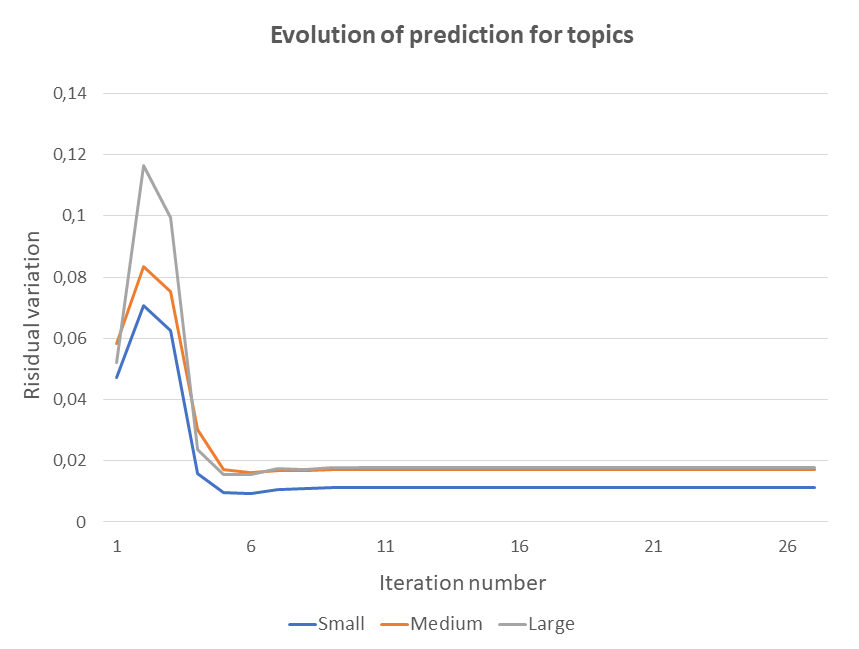
\includegraphics[width=\linewidth]{figs/total}}
	\caption{Algorithm convergence for all topics} 
	\label{fig:converge}
\end{figure}


\subsection{Timeliness}
We evaluate the time execution of the algorithm in order to study how the model of theory of mind evolves.For each dialogue, we computed the time excution of the negotiation. Results are presented in table \ref{tab:time}, where wee see the evolution of the time execution. Unfortunatly, the evolution of the algorithm is exponential.

%	\begin{figure*}[t]
%		\minipage{0.3\textwidth}
%		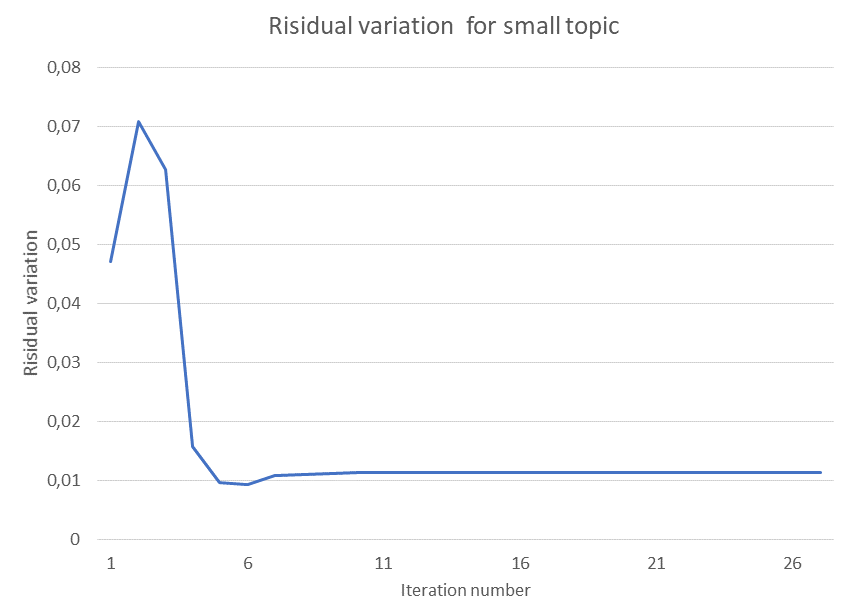
\includegraphics[width=\linewidth]{figs/small.png}
%		\caption{A really Awesome Image}\label{fig:small}
%		\endminipage\hfill
%		\minipage{0.3\textwidth}
%		\fbox{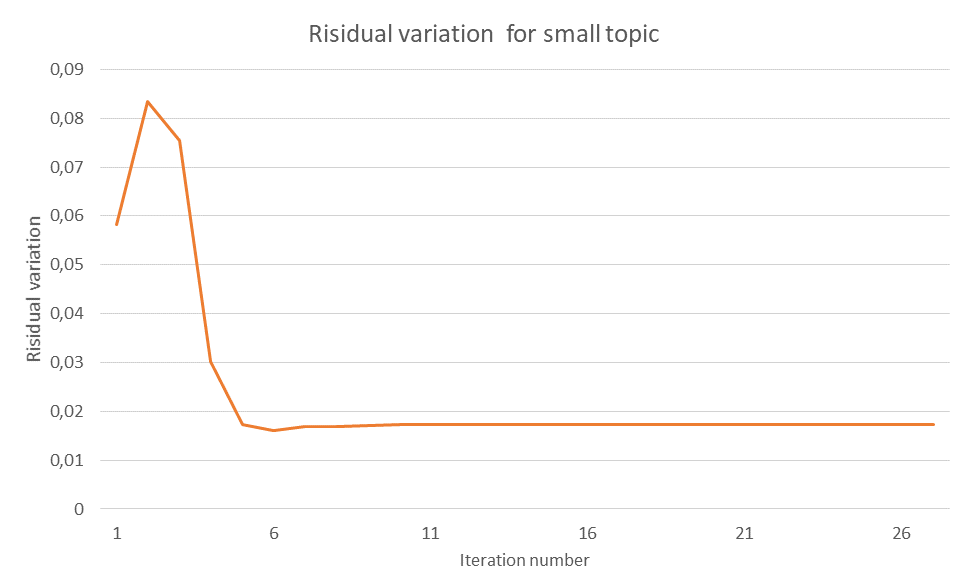
\includegraphics[width=\linewidth]{figs/medium.png}}
%		\caption{A really Awesome Image}\label{fig:medium}
%		\endminipage\hfill
%		\minipage{0.3\textwidth}%
%		\fbox{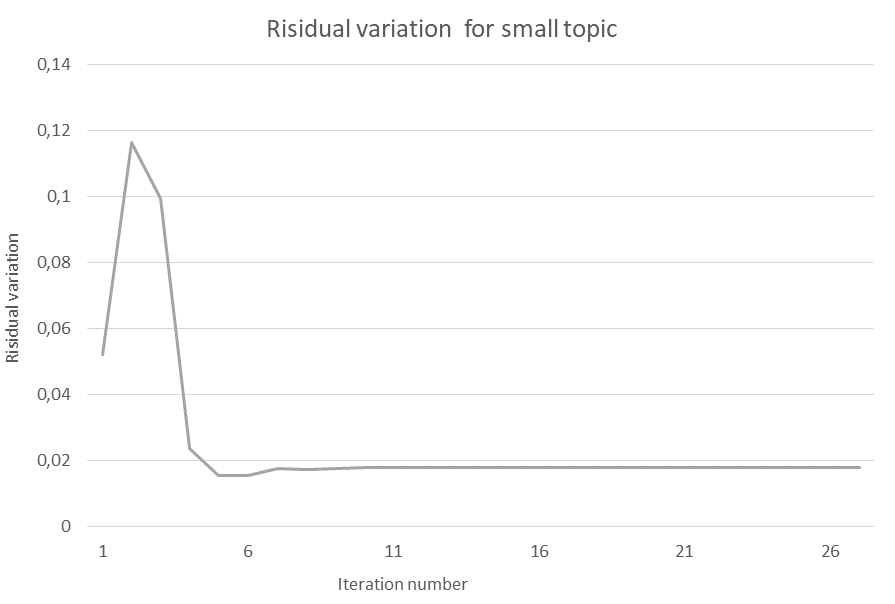
\includegraphics[width=\linewidth]{figs/large.png}}
%		\caption{A really Awesome Image}\label{fig:large}
%		\endminipage
%	\end{figure*}
%	
\section{Discussion}
The results show that agents with theory of mind abilities were able to correctly predict the other agent's behaviors of power

\section{Conclusion}
%%%%%%%%%%%%%%%%%%%%%%%%%%%%%%%%%%%%%%%%%%%%%%%%%%%%%%%%%%%%%%%%%%%%%%%%%%%%%%%%%%%%%%%%%%%%%%%%%%%%%%%%%
%% bibliography: see CFP for number of permitted pages

\bibliographystyle{IEEEtran}
% argument is your BibTeX string definitions and bibliography database(s)
\bibliography{IEEEabrv,bibliography}% put name of your .bib file here





% that's all folks
\end{document}


